This project was written as a semester project by group SW702E13 - Software students from the Department of Computer Science at Aalborg University in the Autumn of 2013. The report documents the implementation of Exhib application and website. The application is developed for the Android platform. The reader is expected to be familiar with Java and the Android platform. We have included our knowledge from all our previous semesters.
\\\\
When reading the report, there are a few things the reader should be aware of:
\begin{itemize}
\item When a reference to a source of a section or paragraph is given, the number of the source is written inside square brackets $[\;]$. The number is a reference to the bibliography list on page \pageref{chap:bib}.
\item When "we/us/our" is mentioned in the report, it is a referral to the authors of the report
\item In class diagrams a minus symbol denotes a private attribute/method, a plus symbol denotes a public attribute/method, and a sharp symbol denotes a protected attribute/method. Italic class names are abstract classes.
\end{itemize}
\begin{center}
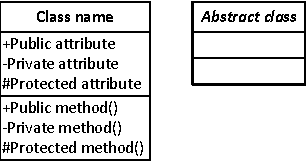
\includegraphics[width=0.35\linewidth]{img/umltheory.pdf}
\end{center}
We would like to thank our supervisor Hua Lu for the feedback he has given throughout the project.
